\documentclass[aspectratio=169,11pt,t,xcolor=table]{beamer}
\usepackage{slidestyle}
\externaldocument[H-]{handout}
% Lesson 1 lost-mark points (from the material plus teaching observation), numbered once
\setcounter{lostmark}{0}
\lostmark{expand}{Differentiating brackets without expanding first: $(2x+1)(x-3)$ is not differentiated factor by factor.}
\lostmark{wrongfn}{Using the wrong function: the \kw{gradient} comes from $f'(x)$, the \kw{$y$-coordinate} comes from $f(x)$.}
\lostmark{terms}{Slips on simple terms: $7x \to 7$ (not $7x$ or $0$), and a constant $\to 0$.}
\lostmark{xinm}{Leaving $x$ inside the tangent's gradient: $y-y_{1}=(4x-3)(x-x_{1})$ is not a straight line. Substitute first.}
\lostmark{signs}{Sign slips with negative $x$: write $(-1)^{2}$ and $(-1)^{3}$ in brackets.}
\lostmark{nocalc}{``Use calculus'' ignored: $f'(x)$ must be written down. A calculator value alone does not show the method.}

\newlength\figunit
\begin{document}

% ------------------------------------------------------------------
\begin{frame}{Lesson 1 \textperiodcentered\ Gradients, Differentiation and Tangents}\relax
\vskip6mm
{\sEmph\bfseries Learning intention\par}\vskip2mm
Differentiate polynomials, and use $f'(x)$ to find the gradient of a curve and the equation of a tangent.
\vskip6mm
{\sEmph\bfseries Success looks like\par}\vskip2mm
\begin{itemize}
\item I can differentiate any polynomial, expanding brackets first.
\item I can choose: gradient at a point, point with a gradient, or unknown constant.
\item I can write the equation of a tangent in three steps.
\end{itemize}
\note{Teaching line, not a question slide.\par
Say: calculus is about gradients of curves. Today is the toolkit every later lesson uses.\par
Timing: Do Now 10 min, three teach-and-practise rounds about 20 min each, practice sheet 30 min, wrap-up 5 min.}
\end{frame}

% ------------------------------------------------------------------
\begin{frame}{Do Now}\relax
\begin{columns}[T]
\begin{column}{0.48\textwidth}
\qn{1} Find the gradient of the line through $(1,\,3)$ and $(4,\,12)$.
\vskip5mm
\qn{2} Expand and simplify $3x(x-4)$.
\end{column}
\begin{column}{0.48\textwidth}
\qn{3} Find the equation of the line with gradient $-2$ that passes through $(3,\,5)$.
\vskip5mm
\qn{4} Solve $x^{2}-5x+6=0$.
\end{column}
\end{columns}
\sfoot{Prerequisites}
\note{Q1 $3$\par
Q2 $3x^{2}-12x$\par
Q3 $y=-2x+11$\par
Q4 $x=2$ or $x=3$\par
Short solution:\par
Q1 $m=\dfrac{12-3}{4-1}=\dfrac{9}{3}=3$\par
Q2 $3x\times x-3x\times4$\par
Q3 $y-5=-2(x-3)$, so $y=-2x+6+5$\par
Q4 $(x-2)(x-3)=0$\par
Watch for:\par
Q1 run over rise gives $\dfrac{1}{3}$\par
Q3 sign error when expanding $-2(x-3)$\par
Diagnostic:\par
Q1 wrong: gradient idea is shaky; spend longer on the one-idea slide\par
Q2 wrong: expect L1 errors (expanding before differentiating)\par
Q3 wrong: the tangent step (round 3) will fail; re-teach $y-y_{1}=m(x-x_{1})$ first\par
Q4 wrong: allow the calculator EQUA menu for quadratics today}
\end{frame}

% ------------------------------------------------------------------
\begin{frame}{The one idea}\relax
\begin{columns}[c]
\begin{column}{0.50\textwidth}
A curve's steepness changes from point to point.
\vskip3mm
The gradient of a curve at a point $=$ the gradient of its \kw{tangent} there.
\vskip3mm
\kw{$f'(x)$ is a gradient machine}: put in $x$, get out the gradient.
\vskip3mm
At A, B and C: going up or down? Which is steepest?
\end{column}
\begin{column}{0.48\textwidth}\centering
\setlength\figunit{10mm}
% y = x^2 with tangents at x = -1, 1, 2.  Tangent at x = a: y = 2a x - a^2 (computed).
% Caller sets \figunit.  Points A, B, C are at x = -1, 1, 2.
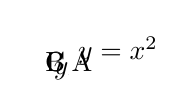
\begin{tikzpicture}[x=\figunit, y=0.6\figunit, line cap=round]
  \gridaxes{-3}{3}{-2}{6}{1}{2}{$y$}
  \begin{scope}
    \clip (-3,-2) rectangle (3,6);
    \curve{-2.5}{2.5}{\x*\x}
    \foreach \a/\pos in {-1/left, 1/right, 2/right}{
      \draw[line width=0.8pt, dashed] ({\a-0.9},{2*\a*(\a-0.9)-\a*\a}) -- ({\a+0.9},{2*\a*(\a+0.9)-\a*\a});
      \fill (\a,{\a*\a}) circle (2.2pt);
    }
  \end{scope}
  \node[anchor=south west] at (2.5,{2.5*2.5-0.2}) {$y=x^{2}$};
  % letters sit inside the parabola, above each tangent (checked):
  % A: x in [-0.95,-0.6], y in [1.1,1.9]; curve there is below 0.9 and tangent y=-2x-1 below 0.9
  % B: mirror of A;  C: x in [1.6,1.95], y in [4.1,4.9]; curve needs x > 2.02 at y = 4.1
  \node[anchor=south west, inner sep=1pt] at (-0.95,1.1) {A};
  \node[anchor=south east, inner sep=1pt] at (0.95,1.1) {B};
  \node[anchor=south east, inner sep=1pt] at (1.95,4.1) {C};
\end{tikzpicture}

\end{column}
\end{columns}
\sfoot{\hp{idea}}
\note{A down, gradient $-2$\par
B up, gradient $2$\par
C up and steepest, gradient $4$\par
Short solution:\par
for $y=x^{2}$ the gradient machine is $f'(x)=2x$: $2(-1)=-2$, $2(1)=2$, $2(2)=4$\par
Watch for:\par
students reading steepness from height; C is steeper because the tangent rises faster, not because it is higher}
\end{frame}

% ------------------------------------------------------------------
\begin{frame}{The power rule}\relax
\fbx{\dfrac{\mathrm{d}}{\mathrm{d}x}\bigl(a x^{n}\bigr)=a n\,x^{n-1}}
\vskip2mm
\centering
Multiply by the power, then take 1 off the power. Do each term on its own.
\vskip4mm
\renewcommand{\arraystretch}{1.35}
\begin{tabular}{lccccc}
\toprule
term & $x^{5}$ & $4x^{3}$ & $-6x^{2}$ & $7x$ & $9$\\
\tderiv & & & & & \\
\bottomrule
\end{tabular}
\vskip4mm
\raggedright
\kw{Expand brackets first}: the rule works on single terms only.
\sfoot{\hp{rule}}
\note{$x^{5}\to5x^{4}$\par
$4x^{3}\to12x^{2}$\par
$-6x^{2}\to-12x$\par
$7x\to7$\par
$9\to0$\par
Short solution:\par
$7x=7x^{1}\to7\times1\times x^{0}=7$; a constant is a flat line, gradient $0$\par
Watch for:\par
$7x\to7x$ or $7x\to0$ (L3)\par
the sign travels with the term: $-6x^{2}\to-12x$}
\end{frame}

% ------------------------------------------------------------------
\begin{frame}{Worked examples \textperiodcentered\ differentiate}\relax
\qn{1} Differentiate $f(x)=3x^{4}-5x^{2}+7x-2$.
\vskip1mm
\hspace*{6mm}Step 1: term by term\qquad Step 2: $f'(x)=\ \ldots$
\vskip6mm
\qn{2} Differentiate $y=(2x+1)(x-3)$.
\vskip1mm
\hspace*{6mm}Step 1: expand\qquad Step 2: $\dydx=\ \ldots$
\sfoot{\hp{rule}}
\note{Q1 $f'(x)=12x^{3}-10x+7$\par
Q2 $\dfrac{dy}{dx}=4x-5$\par
Short solution:\par
Q1 $3x^{4}\to12x^{3}$, $-5x^{2}\to-10x$, $7x\to7$, $-2\to0$\par
Q2 $y=2x^{2}-6x+x-3=2x^{2}-5x-3$\par
Watch for:\par
Q2 differentiating each bracket and multiplying gives $2\times1=2$ (L1)}
\end{frame}

% ------------------------------------------------------------------
\begin{frame}{Practice}\relax
Differentiate.
\vskip4mm
\qn{1} $f(x)=5x^{3}-4x^{2}+x-9$
\vskip5mm
\qn{2} $y=x(x^{2}+6)$
\vskip5mm
\qn{3} $y=(x-2)^{2}$
\sfoot{\hp{rule}}
\note{Q1 $f'(x)=15x^{2}-8x+1$\par
Q2 $\dfrac{dy}{dx}=3x^{2}+6$\par
Q3 $\dfrac{dy}{dx}=2x-4$\par
Short solution:\par
Q2 expand: $y=x^{3}+6x$\par
Q3 expand: $(x-2)^{2}=x^{2}-4x+4$\par
Watch for:\par
Q3 $(x-2)^{2}\ne x^{2}+4$; the middle term $-4x$ is the one that matters\par
Q1 the $x$-term gives $1$, not $0$}
\end{frame}

% ------------------------------------------------------------------
\begin{frame}{Three question types}\relax
\renewcommand{\arraystretch}{1.45}
\begin{tabular}{@{}p{55mm}p{97mm}@{}}
\toprule
given $\to$ asked & route\\
\midrule
$x$ $\to$ gradient & differentiate, then \kw{substitute $x$ into $f'(x)$}\\
gradient $\to$ point & solve $f'(x)=$ gradient for $x$; then $y$ from $f(x)$\\
gradient at $x$ $\to$ constant & differentiate with the letter in; substitute $x$; solve\\
\bottomrule
\end{tabular}
\vskip5mm
The \kw{gradient} comes from $f'(x)$. The $y$-coordinate comes from $f(x)$.
\sfoot{\hp{types}}
\note{Teaching line, not a question slide.\par
Ask the student to underline what is given and circle what is asked before choosing a row.\par
L2 (substituting into the wrong function) is the most common slip in this lesson.}
\end{frame}

% ------------------------------------------------------------------
\begin{frame}{Worked examples \textperiodcentered\ gradients}\relax
\qn{3} Find the gradient of $f(x)=x^{3}-6x^{2}+4$ at the point where $x=5$.
\vskip5mm
\qn{4} Find the point on $y=x^{2}-7x+1$ where the gradient is $3$.
\vskip5mm
\qn{5} The curve $f(x)=ax^{2}+3x-1$ has gradient $11$ at $x=2$. Find $a$.
\sfoot{\hp{types}}
\note{Q3 $15$\par
Q4 $(5,\,-9)$\par
Q5 $a=2$\par
Short solution:\par
Q3 $f'(x)=3x^{2}-12x$; $f'(5)=75-60$\par
Q4 $2x-7=3$ gives $x=5$; $y=25-35+1$\par
Q5 $f'(x)=2ax+3$; $4a+3=11$\par
Watch for:\par
Q4 stopping at $x=5$: a point needs $y$ as well\par
Q5 differentiating $a$ away; $a$ is a number and stays}
\end{frame}

% ------------------------------------------------------------------
\begin{frame}{Practice}\relax
\qn{1} Find the gradient of $f(x)=2x^{3}+x^{2}-4x$ at the point where $x=2$.
\vskip5mm
\qn{2} Find the coordinates of the point on $y=x^{2}+4x-3$ where the gradient is $10$.
\vskip5mm
\qn{3} The curve $f(x)=kx^{3}-2x$ has gradient $22$ when $x=2$. Find $k$.
\sfoot{\hp{types}}
\note{Q1 $24$\par
Q2 $(3,\,18)$\par
Q3 $k=2$\par
Short solution:\par
Q1 $f'(x)=6x^{2}+2x-4$; $f'(2)=24+4-4$\par
Q2 $2x+4=10$ gives $x=3$; $y=9+12-3$\par
Q3 $f'(x)=3kx^{2}-2$; $12k-2=22$\par
Watch for:\par
Q1 substituting into $f(x)$ gives $16$ (L2)\par
Q3 $3kx^{2}$ at $x=2$ is $12k$, not $6k$}
\end{frame}

% ------------------------------------------------------------------
\begin{frame}{Equation of a tangent}\relax
{\sEmph\bfseries Write it in this order\par}\vskip2mm
\begin{enumerate}
\item \kw{Point}: $y_{1}$ from $f(x)$.
\item \kw{Gradient}: $m=f'(x_{1})$, a number.
\item Line: $y-y_{1}=m(x-x_{1})$, then $y=mx+c$.
\end{enumerate}
\vskip4mm
\qn{6} Find the equation of the tangent to $y=x^{3}-2x+1$ at $x=2$.
\sfoot{\hp{tangent}}
\note{Q6 $y=10x-15$\par
Short solution:\par
Q6 point $(2,\,5)$; $\dfrac{dy}{dx}=3x^{2}-2$, $m=10$; $y-5=10(x-2)$\par
Watch for:\par
using $f'(x)$ for $y_{1}$ gives $(2,\,10)$ (L2)\par
writing $y-5=(3x^{2}-2)(x-2)$: the gradient must be a number (L4)}
\end{frame}

% ------------------------------------------------------------------
\begin{frame}{Worked example \textperiodcentered\ two unknowns}\relax
\qn{7} The curve $y=ax^{2}+bx$ passes through $(1,\,5)$, and its gradient at that point is $8$. Find $a$ and $b$.
\vskip3mm
\hspace*{6mm}one equation from the \kw{point}\quad $+$\quad one from the \kw{gradient}
\vskip7mm
Parallel lines have equal gradients:\\[1mm]
``tangent parallel to $y=2x+1$'' means $f'(x)=2$.
\sfoot{\hp{tangent}}
\note{Q7 $a=3$, $b=2$\par
Short solution:\par
Q7 point: $a+b=5$; gradient: $2a+b=8$; subtract: $a=3$\par
Watch for:\par
Q7 using only one condition and guessing the other letter\par
Merit marker: two linked conditions, clearly labelled}
\end{frame}

% ------------------------------------------------------------------
\begin{frame}{Practice}\relax
\qn{1} Find the equation of the tangent to $f(x)=2x^{2}-3x+4$ at $x=2$.
\vskip5mm
\qn{2} The tangent to $y=x^{2}-4x+7$ at the point P is parallel to the line $y=2x+1$. Find the equation of this tangent.
\vskip5mm
\qn{3} The tangent to $y=x^{3}$ at $x=1$ meets the curve again. Find the coordinates of this second point.
\sfoot{\hp{tangent}}
\note{Q1 $y=5x-4$\par
Q2 $y=2x-2$\par
Q3 $(-2,\,-8)$\par
Short solution:\par
Q1 point $(2,\,6)$; $f'(x)=4x-3$, $m=5$; $y-6=5(x-2)$\par
Q2 $2x-4=2$ gives $x=3$; point $(3,\,4)$; $y-4=2(x-3)$\par
Q3 tangent $y=3x-2$; $x^{3}-3x+2=0$; $(x-1)^{2}(x+2)=0$, so $x=-2$\par
Watch for:\par
Q2 the point P is not given: find it from the gradient first (Merit)\par
Q3 Excellence stretch; the repeated root $x=1$ is the point of contact}
\end{frame}

% ------------------------------------------------------------------
\begin{frame}{Ways to lose marks}\relax
\begin{itemize}
\item[\lmnum{expand}] Not expanding brackets before differentiating.
\item[\lmnum{wrongfn}] Gradient from $f'(x)$; $y$-coordinate from $f(x)$.
\item[\lmnum{terms}] $7x\to7$ and a constant $\to0$.
\item[\lmnum{xinm}] The tangent's gradient must be a number, not $f'(x)$.
\item[\lmnum{nocalc}] ``Use calculus'': write $f'(x)$ down.
\end{itemize}
\sfoot{\hp{lose}}
\note{Teaching line, not a question slide.\par
Full list L1 to L6 is in the handout; L5 (brackets around negative $x$) is there too.\par
Ask: which of these did you do today? Tick them in the handout.}
\end{frame}

% ------------------------------------------------------------------
\begin{frame}{Summary}\relax
{\sSum
\begin{enumerate}
\item $\dfrac{\mathrm{d}}{\mathrm{d}x}(ax^{n})=anx^{n-1}$; expand brackets first.
\item Gradient at a point: substitute $x$ into $f'(x)$.
\item Given a gradient: solve $f'(x)=m$; $y$ from $f(x)$.
\item Tangent: point, gradient, then $y-y_{1}=m(x-x_{1})$.
\end{enumerate}}
\sfoot{\hp{idea}}
\note{Teaching line, not a question slide.\par
Ask the student to say each line back before looking at the screen.}
\end{frame}

% ------------------------------------------------------------------
\begin{frame}{Practice sheet \textperiodcentered\ 30 minutes}\relax
Work alone on the practice sheet.
\vskip3mm
\begin{itemize}
\item Questions 1 to 4: warm-up, about 8 minutes.
\item Questions 5 to 10: exam questions, about 22 minutes.
\item Show every line of working; write $f'(x)$ each time.
\end{itemize}
\vskip3mm
Stuck for more than 3 minutes? Move on and come back.
\sfoot{Practice sheet}
\note{Q1 $f'(x)=24x^{3}-9x^{2}+2$\par
Q2 $11$\par
Q3 $(3,\,-7)$\par
Q4 $y=9x-25$\par
Q5 $89$\par
Q6 $y=6.5x-8$\par
Q7 $c=4$\par
Q8 $204$\par
Q9 $p=-4$, $q=0.5$\par
Q10 $y=-2x-2$\par
Short solution:\par
Q6 point $(2,\,5)$; $f'(x)=1.5x^{2}+0.5$, $m=6.5$\par
Q7 $f'(x)=3+2cx-6x^{2}$; $f'(2)=4c-21=-5$\par
Q9 point: $2p-4q=-10$; gradient: $p-4q=-6$; subtract: $p=-4$\par
Q10 expand $y=2x^{2}-6x$; point $(1,\,-4)$; $m=4-6=-2$\par
Watch for:\par
Q6 halves: keep $\dfrac{1}{2}x^{3}\to\dfrac{3}{2}x^{2}$\par
Q10 must expand first (L1)\par
Full working: practice answer version (tutor's working, not an official mark scheme)}
\end{frame}

% ------------------------------------------------------------------
\begin{frame}{Homework}\relax
{\sEmph\bfseries Homework sheet: 15 questions, about 60 minutes\par}
\vskip4mm
\begin{itemize}
\item Questions 1 to 12: Achieved practice.
\item Questions 13 and 14: Merit.
\item Question 15: Extension (Excellence).
\end{itemize}
\vskip4mm
Optional extra: StudyTime Guide, ``Stop and Check'' on pages 10 and 12.
\sfoot{Homework}
\note{Teaching line, not a question slide.\par
Answers: homework answer version (tutor's working, not an official mark scheme).\par
Next lesson Do Now checks Q2 style (differentiate after expanding) and gradient at a point.}
\end{frame}
\end{document}
